\documentclass{extbook}[14pt]
\usepackage{multicol, enumerate, enumitem, hyperref, color, soul, setspace, parskip, fancyhdr, amssymb, amsthm, amsmath, bbm, latexsym, units, mathtools}
\everymath{\displaystyle}
\usepackage[headsep=0.5cm,headheight=0cm, left=1 in,right= 1 in,top= 1 in,bottom= 1 in]{geometry}
\usepackage{dashrule}  % Package to use the command below to create lines between items
\newcommand{\litem}[1]{\item #1

\rule{\textwidth}{0.4pt}}
\pagestyle{fancy}
\lhead{}
\chead{Answer Key for Progress Quiz 3 Version A}
\rhead{}
\lfoot{3148-2249}
\cfoot{}
\rfoot{Spring 2021}
\begin{document}
\textbf{This key should allow you to understand why you choose the option you did (beyond just getting a question right or wrong). \href{https://xronos.clas.ufl.edu/mac1105spring2020/courseDescriptionAndMisc/Exams/LearningFromResults}{More instructions on how to use this key can be found here}.}

\textbf{If you have a suggestion to make the keys better, \href{https://forms.gle/CZkbZmPbC9XALEE88}{please fill out the short survey here}.}

\textit{Note: This key is auto-generated and may contain issues and/or errors. The keys are reviewed after each exam to ensure grading is done accurately. If there are issues (like duplicate options), they are noted in the offline gradebook. The keys are a work-in-progress to give students as many resources to improve as possible.}

\rule{\textwidth}{0.4pt}

\begin{enumerate}\litem{
Construct the lowest-degree polynomial given the zeros below. Then, choose the intervals that contain the coefficients of the polynomial in the form $x^3+bx^2+cx+d$.
\[ 5 + 3 i \text{ and } -3 \]

The solution is \( x^{3} -7 x^{2} +4 x + 102 \), which is option B.\begin{enumerate}[label=\Alph*.]
\item \( b \in [7, 11], c \in [2.8, 4.9], \text{ and } d \in [-111, -99] \)

$x^{3} +7 x^{2} +4 x -102$, which corresponds to multiplying out $(x-(5 + 3 i))(x-(5 - 3 i))(x -3)$.
\item \( b \in [-13, -3], c \in [2.8, 4.9], \text{ and } d \in [92, 105] \)

* $x^{3} -7 x^{2} +4 x + 102$, which is the correct option.
\item \( b \in [-5, 2], c \in [-5.1, -1], \text{ and } d \in [-19, -11] \)

$x^{3} + x^{2} -2 x -15$, which corresponds to multiplying out $(x -5)(x + 3)$.
\item \( b \in [-5, 2], c \in [-1.5, 3.7], \text{ and } d \in [-13, -7] \)

$x^{3} + x^{2} -9$, which corresponds to multiplying out $(x -3)(x + 3)$.
\item \( \text{None of the above.} \)

This corresponds to making an unanticipated error or not understanding how to use nonreal complex numbers to create the lowest-degree polynomial. If you chose this and are not sure what you did wrong, please contact the coordinator for help.
\end{enumerate}

\textbf{General Comment:} Remember that the conjugate of $a+bi$ is $a-bi$. Since these zeros always come in pairs, we need to multiply out $(x-(5 + 3 i))(x-(5 - 3 i))(x-(-3))$.
}
\litem{
Construct the lowest-degree polynomial given the zeros below. Then, choose the intervals that contain the coefficients of the polynomial in the form $ax^3+bx^2+cx+d$.
\[ \frac{-5}{3}, \frac{7}{2}, \text{ and } \frac{3}{5} \]

The solution is \( 30x^{3} -73 x^{2} -142 x + 105 \), which is option D.\begin{enumerate}[label=\Alph*.]
\item \( a \in [30, 34], b \in [-76, -69], c \in [-148, -138], \text{ and } d \in [-107, -100] \)

$30x^{3} -73 x^{2} -142 x -105$, which corresponds to multiplying everything correctly except the constant term.
\item \( a \in [30, 34], b \in [68, 75], c \in [-148, -138], \text{ and } d \in [-107, -100] \)

$30x^{3} +73 x^{2} -142 x -105$, which corresponds to multiplying out $(3x -5)(2x + 7)(5x + 3)$.
\item \( a \in [30, 34], b \in [-174, -166], c \in [267, 273], \text{ and } d \in [-107, -100] \)

$30x^{3} -173 x^{2} +268 x -105$, which corresponds to multiplying out $(3x -5)(2x -7)(5x -3)$.
\item \( a \in [30, 34], b \in [-76, -69], c \in [-148, -138], \text{ and } d \in [104, 107] \)

* $30x^{3} -73 x^{2} -142 x + 105$, which is the correct option.
\item \( a \in [30, 34], b \in [36, 39], c \in [-208, -198], \text{ and } d \in [104, 107] \)

$30x^{3} +37 x^{2} -208 x + 105$, which corresponds to multiplying out $(3x -5)(2x + 7)(5x -3)$.
\end{enumerate}

\textbf{General Comment:} To construct the lowest-degree polynomial, you want to multiply out $(3x + 5)(2x -7)(5x -3)$
}
\litem{
Which of the following equations \textit{could} be of the graph presented below?

\begin{center}
    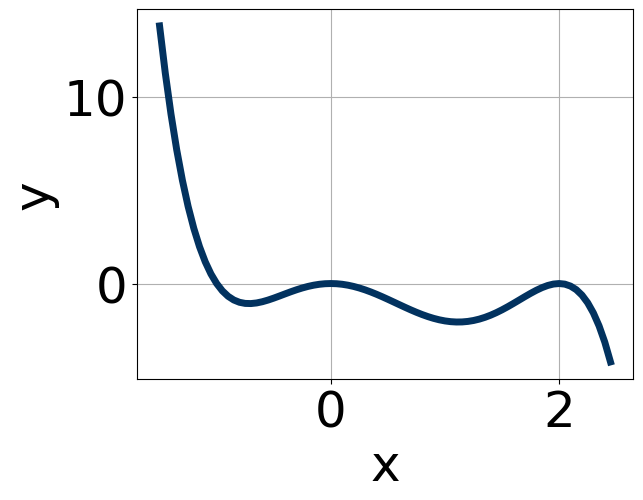
\includegraphics[width=0.5\textwidth]{../Figures/polyGraphToFunctionA.png}
\end{center}




The solution is \( -14x^{6} (x - 2)^{10} (x + 1)^{9} \), which is option A.\begin{enumerate}[label=\Alph*.]
\item \( -14x^{6} (x - 2)^{10} (x + 1)^{9} \)

* This is the correct option.
\item \( 6x^{6} (x - 2)^{8} (x + 1)^{11} \)

This corresponds to the leading coefficient being the opposite value than it should be.
\item \( 20x^{10} (x - 2)^{6} (x + 1)^{8} \)

The factor $(x + 1)$ should have an odd power and the leading coefficient should be the opposite sign.
\item \( -4x^{10} (x - 2)^{5} (x + 1)^{9} \)

The factor $(x - 2)$ should have an even power.
\item \( -8x^{10} (x - 2)^{7} (x + 1)^{8} \)

The factor $(x - 2)$ should have an even power and the factor $(x + 1)$ should have an odd power.
\end{enumerate}

\textbf{General Comment:} General Comments: Draw the x-axis to determine which zeros are touching (and so have even multiplicity) or cross (and have odd multiplicity).
}
\litem{
Describe the end behavior of the polynomial below.
\[ f(x) = -9(x + 5)^{3}(x - 5)^{6}(x + 2)^{2}(x - 2)^{4} \]

The solution is the graph below, which is option A.
\begin{center}
    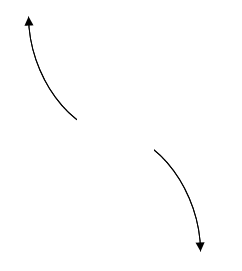
\includegraphics[width=0.3\textwidth]{../Figures/polyEndBehaviorCopyAA.png}
\end{center}\begin{enumerate}[label=\Alph*.]
\begin{multicols}{2}
\item 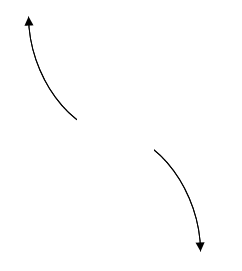
\includegraphics[width = 0.3\textwidth]{../Figures/polyEndBehaviorCopyAA.png}
\item 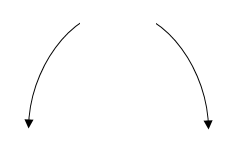
\includegraphics[width = 0.3\textwidth]{../Figures/polyEndBehaviorCopyBA.png}
\item 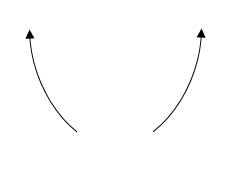
\includegraphics[width = 0.3\textwidth]{../Figures/polyEndBehaviorCopyCA.png}
\item 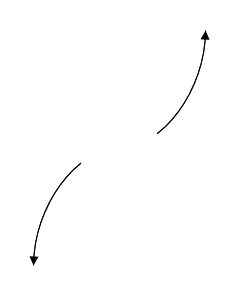
\includegraphics[width = 0.3\textwidth]{../Figures/polyEndBehaviorCopyDA.png}
\end{multicols}\item None of the above.\end{enumerate}
\textbf{General Comment:} Remember that end behavior is determined by the leading coefficient AND whether the \textbf{sum} of the multiplicities is positive or negative.
}
\litem{
Construct the lowest-degree polynomial given the zeros below. Then, choose the intervals that contain the coefficients of the polynomial in the form $ax^3+bx^2+cx+d$.
\[ 1, 5, \text{ and } \frac{-3}{5} \]

The solution is \( 5x^{3} -27 x^{2} +7 x + 15 \), which is option D.\begin{enumerate}[label=\Alph*.]
\item \( a \in [4, 15], b \in [32, 36], c \in [41, 45], \text{ and } d \in [10, 17] \)

$5x^{3} +33 x^{2} +43 x + 15$, which corresponds to multiplying out $(x + 1)(x + 5)(5x + 3)$.
\item \( a \in [4, 15], b \in [19, 30], c \in [1, 17], \text{ and } d \in [-17, -11] \)

$5x^{3} +27 x^{2} +7 x -15$, which corresponds to multiplying out $(x + 1)(x + 5)(5x -3)$.
\item \( a \in [4, 15], b \in [-24, -14], c \in [-50, -34], \text{ and } d \in [-17, -11] \)

$5x^{3} -17 x^{2} -37 x -15$, which corresponds to multiplying out $(x + 1)(x -5)(5x + 3)$.
\item \( a \in [4, 15], b \in [-33, -26], c \in [1, 17], \text{ and } d \in [10, 17] \)

* $5x^{3} -27 x^{2} +7 x + 15$, which is the correct option.
\item \( a \in [4, 15], b \in [-33, -26], c \in [1, 17], \text{ and } d \in [-17, -11] \)

$5x^{3} -27 x^{2} +7 x -15$, which corresponds to multiplying everything correctly except the constant term.
\end{enumerate}

\textbf{General Comment:} To construct the lowest-degree polynomial, you want to multiply out $(x -1)(x -5)(5x + 3)$
}
\litem{
Which of the following equations \textit{could} be of the graph presented below?

\begin{center}
    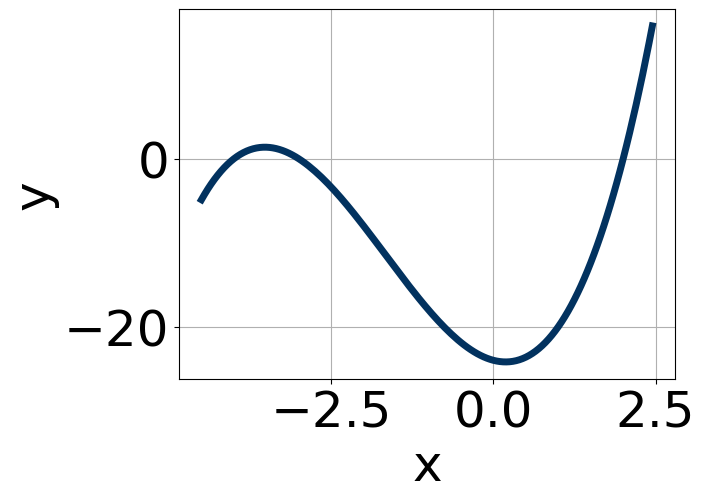
\includegraphics[width=0.5\textwidth]{../Figures/polyGraphToFunctionCopyA.png}
\end{center}




The solution is \( 14(x - 2)^{11} (x - 3)^{5} (x + 4)^{5} \), which is option A.\begin{enumerate}[label=\Alph*.]
\item \( 14(x - 2)^{11} (x - 3)^{5} (x + 4)^{5} \)

* This is the correct option.
\item \( -6(x - 2)^{5} (x - 3)^{9} (x + 4)^{11} \)

This corresponds to the leading coefficient being the opposite value than it should be.
\item \( 4(x - 2)^{6} (x - 3)^{5} (x + 4)^{11} \)

The factor $2$ should have been an odd power.
\item \( 7(x - 2)^{10} (x - 3)^{10} (x + 4)^{7} \)

The factors $2$ and $3$ have have been odd power.
\item \( -15(x - 2)^{4} (x - 3)^{9} (x + 4)^{5} \)

The factor $(x - 2)$ should have an odd power and the leading coefficient should be the opposite sign.
\end{enumerate}

\textbf{General Comment:} General Comments: Draw the x-axis to determine which zeros are touching (and so have even multiplicity) or cross (and have odd multiplicity).
}
\litem{
Describe the zero behavior of the zero $x = -9$ of the polynomial below.
\[ f(x) = 5(x + 4)^{12}(x - 4)^{8}(x - 9)^{9}(x + 9)^{8} \]

The solution is the graph below, which is option B.
\begin{center}
    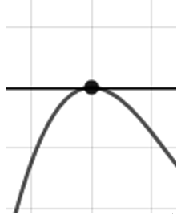
\includegraphics[width=0.3\textwidth]{../Figures/polyZeroBehaviorBA.png}
\end{center}\begin{enumerate}[label=\Alph*.]
\begin{multicols}{2}
\item 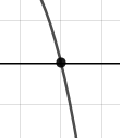
\includegraphics[width = 0.3\textwidth]{../Figures/polyZeroBehaviorAA.png}
\item 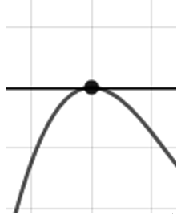
\includegraphics[width = 0.3\textwidth]{../Figures/polyZeroBehaviorBA.png}
\item 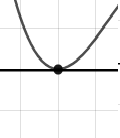
\includegraphics[width = 0.3\textwidth]{../Figures/polyZeroBehaviorCA.png}
\item 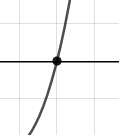
\includegraphics[width = 0.3\textwidth]{../Figures/polyZeroBehaviorDA.png}
\end{multicols}\item None of the above.\end{enumerate}
\textbf{General Comment:} You will need to sketch the entire graph, then zoom in on the zero the question asks about.
}
\litem{
Construct the lowest-degree polynomial given the zeros below. Then, choose the intervals that contain the coefficients of the polynomial in the form $x^3+bx^2+cx+d$.
\[ 4 - 5 i \text{ and } 4 \]

The solution is \( x^{3} -12 x^{2} +73 x -164 \), which is option D.\begin{enumerate}[label=\Alph*.]
\item \( b \in [1, 11], c \in [-11, 0], \text{ and } d \in [10, 17] \)

$x^{3} + x^{2} -8 x + 16$, which corresponds to multiplying out $(x -4)(x -4)$.
\item \( b \in [3, 13], c \in [71, 75], \text{ and } d \in [163, 167] \)

$x^{3} +12 x^{2} +73 x + 164$, which corresponds to multiplying out $(x-(4 - 5 i))(x-(4 + 5 i))(x + 4)$.
\item \( b \in [1, 11], c \in [-2, 6], \text{ and } d \in [-27, -17] \)

$x^{3} + x^{2} +x -20$, which corresponds to multiplying out $(x + 5)(x -4)$.
\item \( b \in [-16, -8], c \in [71, 75], \text{ and } d \in [-165, -163] \)

* $x^{3} -12 x^{2} +73 x -164$, which is the correct option.
\item \( \text{None of the above.} \)

This corresponds to making an unanticipated error or not understanding how to use nonreal complex numbers to create the lowest-degree polynomial. If you chose this and are not sure what you did wrong, please contact the coordinator for help.
\end{enumerate}

\textbf{General Comment:} Remember that the conjugate of $a+bi$ is $a-bi$. Since these zeros always come in pairs, we need to multiply out $(x-(4 - 5 i))(x-(4 + 5 i))(x-(4))$.
}
\litem{
Describe the zero behavior of the zero $x = 9$ of the polynomial below.
\[ f(x) = 4(x + 9)^{8}(x - 9)^{9}(x + 8)^{9}(x - 8)^{10} \]

The solution is the graph below, which is option D.
\begin{center}
    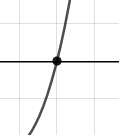
\includegraphics[width=0.3\textwidth]{../Figures/polyZeroBehaviorCopyDA.png}
\end{center}\begin{enumerate}[label=\Alph*.]
\begin{multicols}{2}
\item 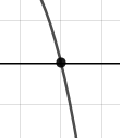
\includegraphics[width = 0.3\textwidth]{../Figures/polyZeroBehaviorCopyAA.png}
\item 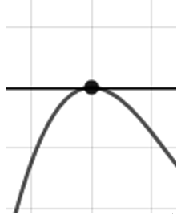
\includegraphics[width = 0.3\textwidth]{../Figures/polyZeroBehaviorCopyBA.png}
\item 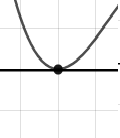
\includegraphics[width = 0.3\textwidth]{../Figures/polyZeroBehaviorCopyCA.png}
\item 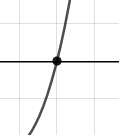
\includegraphics[width = 0.3\textwidth]{../Figures/polyZeroBehaviorCopyDA.png}
\end{multicols}\item None of the above.\end{enumerate}
\textbf{General Comment:} You will need to sketch the entire graph, then zoom in on the zero the question asks about.
}
\litem{
Describe the end behavior of the polynomial below.
\[ f(x) = 2(x - 8)^{4}(x + 8)^{5}(x - 6)^{2}(x + 6)^{3} \]

The solution is the graph below, which is option C.
\begin{center}
    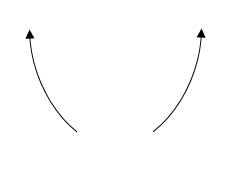
\includegraphics[width=0.3\textwidth]{../Figures/polyEndBehaviorCA.png}
\end{center}\begin{enumerate}[label=\Alph*.]
\begin{multicols}{2}
\item 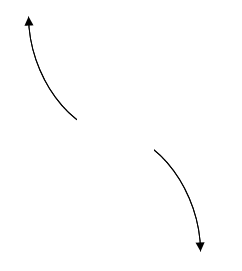
\includegraphics[width = 0.3\textwidth]{../Figures/polyEndBehaviorAA.png}
\item 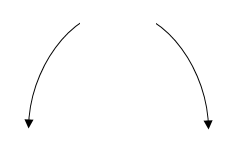
\includegraphics[width = 0.3\textwidth]{../Figures/polyEndBehaviorBA.png}
\item 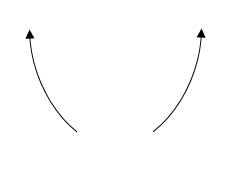
\includegraphics[width = 0.3\textwidth]{../Figures/polyEndBehaviorCA.png}
\item 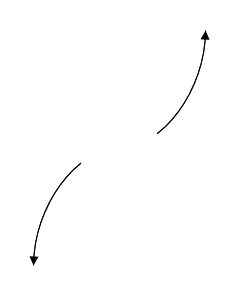
\includegraphics[width = 0.3\textwidth]{../Figures/polyEndBehaviorDA.png}
\end{multicols}\item None of the above.\end{enumerate}
\textbf{General Comment:} Remember that end behavior is determined by the leading coefficient AND whether the \textbf{sum} of the multiplicities is positive or negative.
}
\end{enumerate}

\end{document}